\section{结果}

\subsection{有限局部上下文支持有效词检索}

加入邻近词窗后，检索性能迅速提高；继续扩大上下文，性能趋于饱和，并在部分设置下下降
（图~\ref{fig:word_core_evidence}a,b）。
半径 $2$ 在两个数据集上均取得最高的宏平均 Top-$10$ 种子均值，
相对完整上下文模型在 Pallier2025 和 ChineseEEG-2 上分别提高 $5.10$ 和 $5.12$ 个百分点。
将候选集合扩大到完整训练词库后，局部窗口的 Top-$10$ 优势仍然保留，
但 Top-$1$ 没有一致改善（附录表~\ref{tab:full_vocab_comparison}）。

\begin{figure}[!htbp]
    \centering
    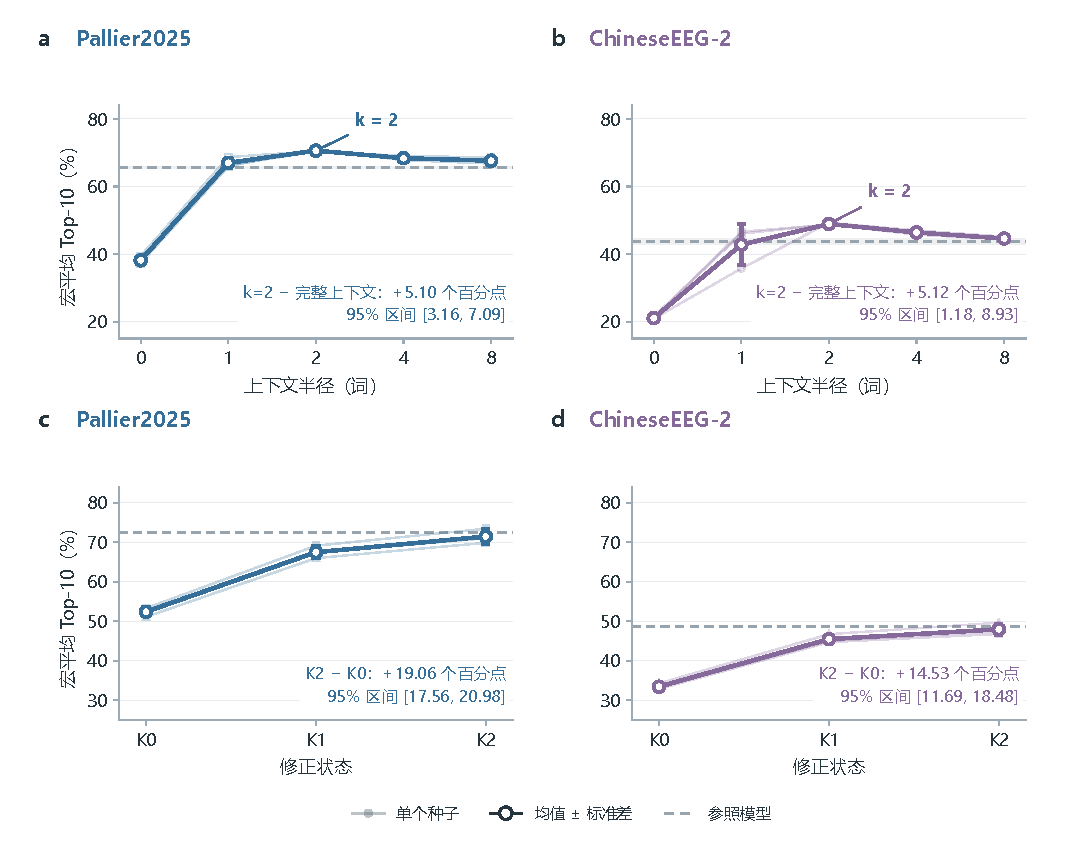
\includegraphics[width=\linewidth]{word_core_with_effects.pdf}
    \caption{词级检索结果（$50$ 词候选，宏平均 Top-$10$）。a,b：不同上下文半径，灰虚线及灰带为完整上下文均值 $\pm$ SD；c,d：共享滚动状态，灰虚线为独立 K2 均值。浅线为单个种子，粗线及误差棒为均值 $\pm$ SD。各面板标出核心差值及 $95\%$ 区间。}
    \label{fig:word_core_evidence}
\end{figure}
\FloatBarrier

\subsection{后续神经输入逐步改善同一目标}

同一目标从 K0 至 K2 的候选排序逐步改善（图~\ref{fig:word_core_evidence}c,d）。
在固定 $50$ 词候选集上，Pallier2025 和 ChineseEEG-2 的宏平均 Top-$10$ 分别提高 $19.06$ 和 $14.53$ 个百分点。
主要改善出现在第一个后续词窗到达之后，第二个后续词窗带来进一步增益；
共享模型的 K2 与单独训练的 K2 具有接近的预测表现，从而使同一组参数可覆盖三个可见状态。

延长单个目标词的观察窗口至 $1.28\,\mathrm{s}$ 或 $1.50\,\mathrm{s}$，并未达到当前跨词模型的词级检索水平（图~\ref{fig:word_controls}）。
该比较同时涉及历史词窗可见性与输入组织方式，因此仅用于说明延长单词输入不能直接替代当前局部上下文设置。
与仅输入目标词的半径 $0$ 模型相比，引入邻近词窗也具有明显的性能优势。

\begin{figure}[!htbp]
    \centering
    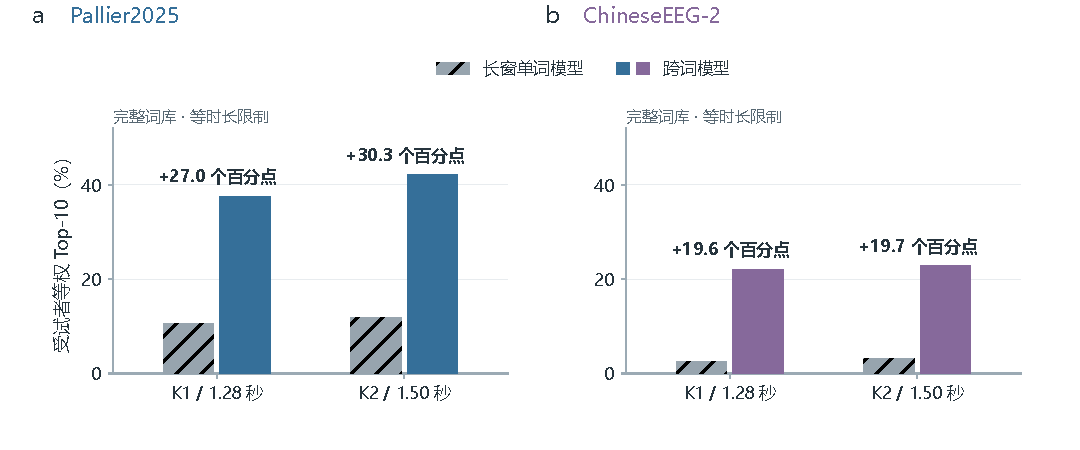
\includegraphics[width=\linewidth]{long_window_comparison.pdf}
    \caption{相近输入可用时刻下的长窗单词模型与局部跨词模型比较。a、b 分别对应 Pallier2025 与 ChineseEEG-2；使用完整训练词库下的受试者等权 Top-$10$。每对结果仅在对应跨词模型的最后输入词窗不晚于长窗结束的共同词位上计算，柱为三个种子的均值，标注为跨词模型减长窗模型的差值。}
    \label{fig:word_controls}
\end{figure}
\FloatBarrier

\subsection{滚动修正的文本收益与输入等待}

\paragraph{法语}
在 Pallier2025 上，滚动修正 C 使平均片段 BLEU-1 从 A 的 $8.37\%$ 提高至 $13.46\%$，
WER 由 $94.94\%$ 降至 $89.11\%$（表~\ref{tab:main}，图~\ref{fig:forest}）。
固定首次 K0 表示、仅重新搜索近期文本的 B，BLEU-1 为 $8.94\%$；
允许历史神经表示更新后，C 比 B 再提高约 $4.52$ 个百分点。
只允许一次回修的 C1 达到 $12.17\%$，平均额外输入等待为 $0.265\,\mathrm{s}$。
在当前序列搜索规则下，表示更新与有限回修能够带来较明确的文本收益。

\paragraph{中文}
ChineseEEG-2 的词级更新同样有效，但序列指标呈现不同结果。
A 到 C 的平均片段 BLEU-1 为 $9.25\%$ 至 $9.76\%$，增益 $+0.51$ 个百分点，
其配对区间 $[-0.41,1.42]$ 跨越零；WER 从 $97.54\%$ 降至 $95.97\%$，
词位准确率从 $2.31\%$ 升至 $3.98\%$。
固定 K0 的文本重搜 B 并未带来相同改善。
中文结果表明，词级候选排序的增益未必同步表现为 BLEU-1 的提高。
C 相对 A、B 的 WER 和词位准确率差异经双侧 Holm 校正后仍成立，具体数值见附录~\ref{sec:supp_statistics}。

\paragraph{与完整片段比较}
Pallier2025 的完整片段策略 F 获得最高 BLEU-1（$15.51\%$）。
在相同整段搜索条件下，F-local 沿用最终局部神经表示，BLEU-1 为 $13.72\%$，
接近 C 的 $13.46\%$；采用完整上下文模型的 F 带来进一步改善。
ChineseEEG-2 上，C、F-local 和 F 的 BLEU-1 差别较小。
C 相对首次预测平均增加 $0.502\,\mathrm{s}$（法语）和 $0.542\,\mathrm{s}$（中文）的输入等待，
比完整片段平均节省 $1.81\,\mathrm{s}$ 和 $1.51\,\mathrm{s}$（图~\ref{fig:tradeoff}）。

\begin{table}[!htbp]
    \centering
    \papertablestyle
    \caption{四种输出策略的平均片段 BLEU-1 与 WER（\%）。完整六策略结果见附录表~\ref{tab:sequence_complete_metrics}。}
    \label{tab:main}
    \label{tab:sentence_revision_full}
    % Presentation only: canonical manuscript_text_stage3_v1 exports.
\begingroup
\papertablestyle
\begin{tabular}{@{}lrrrr@{}}
\toprule
策略 & \multicolumn{2}{c}{Pallier2025} & \multicolumn{2}{c}{ChineseEEG-2} \\
\cmidrule(lr){2-3}\cmidrule(lr){4-5}
 & BLEU-1 $\uparrow$ & WER $\downarrow$ & BLEU-1 $\uparrow$ & WER $\downarrow$ \\
\midrule
A 固定输出 & 8.37 & 94.94 & 9.25 & 97.54 \\
C1 一次回修 & 12.17 & 90.58 & 9.74 & 97.00 \\
C 滚动修正 & 13.46 & 89.11 & 9.76 & 95.97 \\
F 完整片段 & 15.51 & 88.21 & 9.96 & 96.10 \\
\bottomrule
\end{tabular}
\endgroup

\end{table}

\begin{figure}[!htbp]
    \centering
    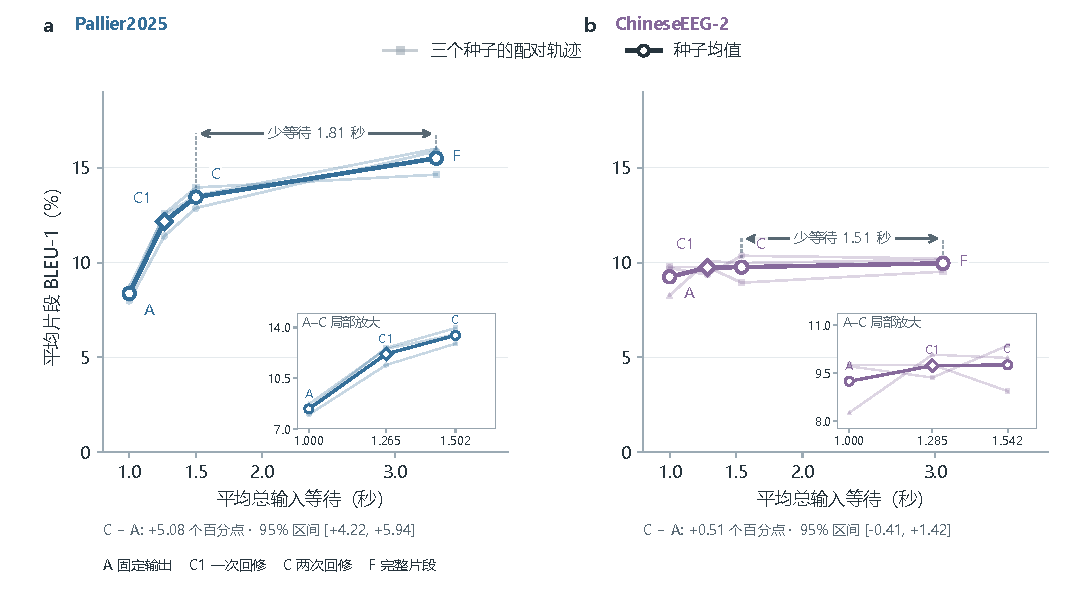
\includegraphics[width=\linewidth]{quality_wait_ac1cf_v2_test.pdf}
    \caption{文本质量与平均总输入等待。浅线为单个种子，空心点为种子均值；插图放大 A/C1/C。箭头为 C 相对 F 的等待节省。总等待包含自身 $1\,\mathrm{s}$ 神经窗。}
    \label{fig:tradeoff}
    \label{fig:sentence_full_context_tradeoff}
\end{figure}

\begin{figure}[!htbp]
    \centering
    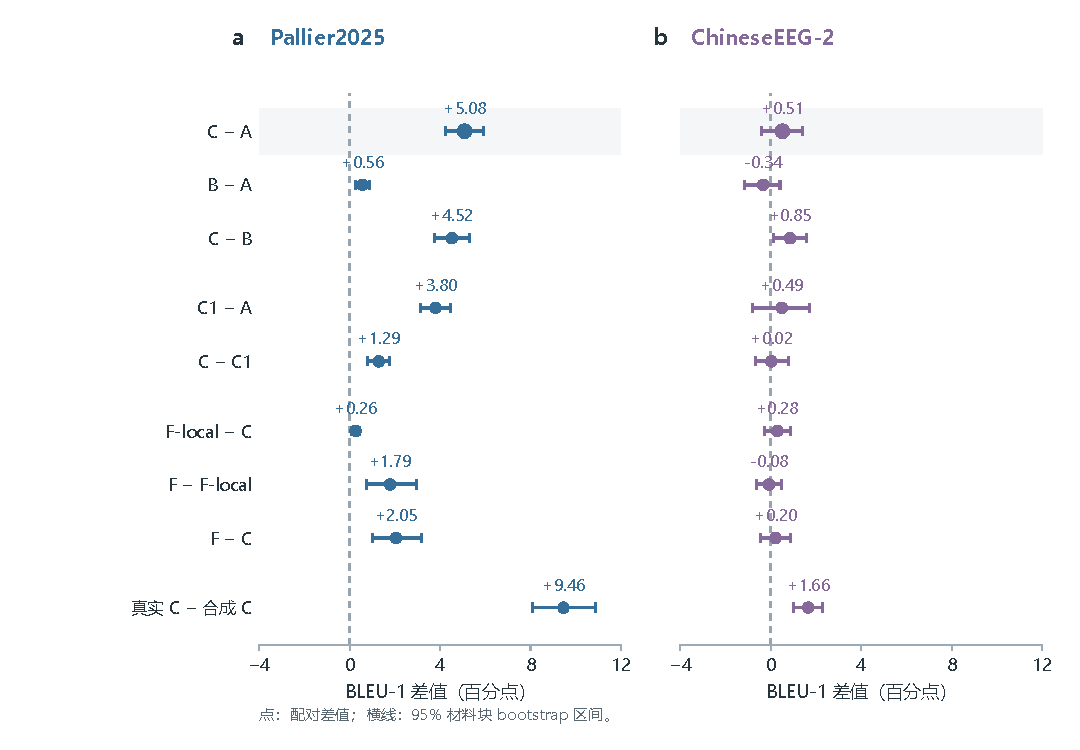
\includegraphics[width=\linewidth]{sequence_effects_forest.pdf}
    \caption{文本策略间的平均片段 BLEU-1 配对差值（百分点）。点为差值，横线为点态 $95\%$ 材料块 bootstrap 区间，虚线表示零；不将点态区间直接解释为多重比较校正后的检验结论。}
    \label{fig:forest}
\end{figure}
\FloatBarrier

\subsection{回修收益与输出稳定性}

从最终词位结果看，回修的净效果为正，改错为对的词位多于改对为错。
但逐次观察时，约 $88$--$94\%$ 的改写发生在错误词之间，最终词位恢复与输出稳定性需要分别评价（图~\ref{fig:sentence_display_edit_composition}；案例见附录图~\ref{fig:sentence_examples_full}）。


\begin{figure}[!htbp]
    \centering
    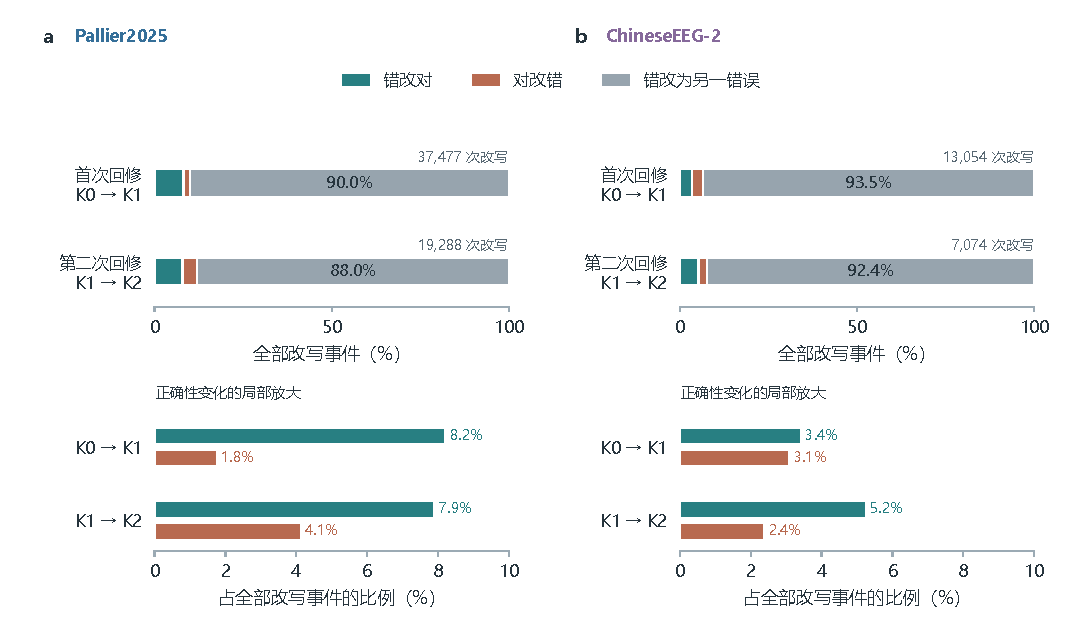
\includegraphics[width=\linewidth]{13_display_edit_composition.pdf}
    \caption{回修事件类型。仅统计输出发生变化的事件，合并三个种子；上排为三类改写组成，下排放大错改对和对改错的比例。}
    \label{fig:sentence_display_edit_composition}
\end{figure}
\FloatBarrier
